\documentclass[onesided]{article}\usepackage[]{graphicx}\usepackage[]{color}
% maxwidth is the original width if it is less than linewidth
% otherwise use linewidth (to make sure the graphics do not exceed the margin)
\makeatletter
\def\maxwidth{ %
  \ifdim\Gin@nat@width>\linewidth
    \linewidth
  \else
    \Gin@nat@width
  \fi
}
\makeatother

\definecolor{fgcolor}{rgb}{0.345, 0.345, 0.345}
\newcommand{\hlnum}[1]{\textcolor[rgb]{0.686,0.059,0.569}{#1}}%
\newcommand{\hlstr}[1]{\textcolor[rgb]{0.192,0.494,0.8}{#1}}%
\newcommand{\hlcom}[1]{\textcolor[rgb]{0.678,0.584,0.686}{\textit{#1}}}%
\newcommand{\hlopt}[1]{\textcolor[rgb]{0,0,0}{#1}}%
\newcommand{\hlstd}[1]{\textcolor[rgb]{0.345,0.345,0.345}{#1}}%
\newcommand{\hlkwa}[1]{\textcolor[rgb]{0.161,0.373,0.58}{\textbf{#1}}}%
\newcommand{\hlkwb}[1]{\textcolor[rgb]{0.69,0.353,0.396}{#1}}%
\newcommand{\hlkwc}[1]{\textcolor[rgb]{0.333,0.667,0.333}{#1}}%
\newcommand{\hlkwd}[1]{\textcolor[rgb]{0.737,0.353,0.396}{\textbf{#1}}}%
\let\hlipl\hlkwb

\usepackage{framed}
\makeatletter
\newenvironment{kframe}{%
 \def\at@end@of@kframe{}%
 \ifinner\ifhmode%
  \def\at@end@of@kframe{\end{minipage}}%
  \begin{minipage}{\columnwidth}%
 \fi\fi%
 \def\FrameCommand##1{\hskip\@totalleftmargin \hskip-\fboxsep
 \colorbox{shadecolor}{##1}\hskip-\fboxsep
     % There is no \\@totalrightmargin, so:
     \hskip-\linewidth \hskip-\@totalleftmargin \hskip\columnwidth}%
 \MakeFramed {\advance\hsize-\width
   \@totalleftmargin\z@ \linewidth\hsize
   \@setminipage}}%
 {\par\unskip\endMakeFramed%
 \at@end@of@kframe}
\makeatother

\definecolor{shadecolor}{rgb}{.97, .97, .97}
\definecolor{messagecolor}{rgb}{0, 0, 0}
\definecolor{warningcolor}{rgb}{1, 0, 1}
\definecolor{errorcolor}{rgb}{1, 0, 0}
\newenvironment{knitrout}{}{} % an empty environment to be redefined in TeX

\usepackage{alltt}
\usepackage[T1]{fontenc}
\linespread{1.5} % Line spacing - Palatino needs more space between lines
\usepackage{microtype} % Slightly tweak font spacing for aesthetics

\usepackage[hmarginratio=1:1,columnsep=20pt]{geometry} % Document margins
%\usepackage{multicol} % Used for the two-column layout of the document
\usepackage[hang, small,labelfont=bf,up,textfont=it,up]{caption} % Custom captions under/above floats in tables or figures
\usepackage{booktabs} % Horizontal rules in tables
\usepackage{float} % Required for tables and figures in the multi-column environment - they need to be placed in specific locations with the [H] (e.g. \begin{table}[H])

\usepackage{lettrine} % The lettrine is the first enlarged letter at the beginning of the text
\usepackage{paralist} % Used for the compactitem environment which makes bullet points with less space between them

% to ignore texts: good for thank messages and paper submissions.
      % \fbox{\phantom{This text will be invisible too, but a box will be printed arround it.}}

\usepackage{abstract} % Allows abstract customization
\renewcommand{\abstractnamefont}{\normalfont\bfseries} % Set the "Abstract" text to bold
%\renewcommand{\abstracttextfont}{\normalfont\small\itshape} % Set the abstract itself to small italic text

\usepackage[]{titlesec} % Allows customization of titles
\renewcommand\thesection{\Roman{section}} % Roman numerals for the sections
\renewcommand\thesubsection{\Roman{subsection}} % Roman numerals for subsections
\titleformat{\section}[block]{\large\scshape\centering}{\thesection.}{1em}{} % Change the look of the section titles
\titleformat{\subsection}[block]{\large}{\thesubsection.}{1em}{} % Change the look of the section titles

\usepackage{fancybox, fancyvrb, calc}
\usepackage[svgnames]{xcolor}
\usepackage{physics}
\usepackage{epigraph}
\usepackage{longtable}
\usepackage{pdflscape}
\usepackage{graphics}
\usepackage{pbox} % \pbox{20cm}{This is the first \\ cell}
\usepackage{amsfonts}
\usepackage{amsmath}
\usepackage{amssymb}
\usepackage{rotating}
\usepackage{paracol}
\usepackage{textcomp}
\usepackage[export]{adjustbox}
\usepackage{afterpage}
\usepackage{filecontents}
\usepackage{color}
\usepackage{latexsym}
\usepackage{lscape}       %\begin{landscape} and \end{landscape}
\usepackage{wasysym}
\usepackage{dashrule}
\usepackage{marvosym} % face package
\usepackage{framed}
\usepackage{tree-dvips}
\usepackage{pgffor}
\usepackage[]{authblk}
\usepackage{setspace}
\usepackage{array}
\usepackage[latin1]{inputenc}
\usepackage{hyperref}     %desactivar para link rojos
\usepackage{graphicx}
\usepackage{dcolumn} % for R tables
\usepackage{multirow} % For multirow in tables
\usepackage{pifont}
\usepackage{listings}
\usepackage{bm}




% hypothesis / theorem package begin
\usepackage{amsthm}
\usepackage{thmtools}
\declaretheoremstyle[
spaceabove=6pt, spacebelow=6pt,
headfont=\normalfont\bfseries,
notefont=\mdseries, notebraces={(}{)},
bodyfont=\normalfont,
postheadspace=0.6em,
headpunct=:
]{mystyle}
\declaretheorem[style=mystyle, name=Hypothesis, preheadhook={\renewcommand{\thehyp}{H\textsubscript{\arabic{hyp}}}}]{hyp}

\usepackage{cleveref}
\crefname{hyp}{hypothesis}{hypotheses}
\Crefname{hyp}{Hypothesis}{Hypotheses}
% hypothesis / theorem package end


%----------------------------------------------------------------------------------------
% Other ADDS-ON
%----------------------------------------------------------------------------------------

% independence symbol \independent
\newcommand\independent{\protect\mathpalette{\protect\independenT}{\perp}}
\def\independenT#1#2{\mathrel{\rlap{$#1#2$}\mkern2mu{#1#2}}}







\hypersetup{
    bookmarks=true,         % show bookmarks bar?
    unicode=false,          % non-Latin characters in Acrobat's bookmarks
    pdftoolbar=true,        % show Acrobat's toolbar?
    pdfmenubar=true,        % show Acrobat's menu?
    pdffitwindow=true,     % window fit to page when opened
    pdfstartview={FitH},    % fits the width of the page to the window
    pdftitle={My title},    % title
    pdfauthor={Author},     % author
    pdfsubject={Subject},   % subject of the document
    pdfcreator={Creator},   % creator of the document
    pdfproducer={Producer}, % producer of the document
    pdfkeywords={keyword1} {key2} {key3}, % list of keywords
    pdfnewwindow=true,      % links in new window
    colorlinks=true,       % false: boxed links; true: colored links
    linkcolor=ForestGreen,          % color of internal links (change box color with linkbordercolor)
    citecolor=ForestGreen,        % color of links to bibliography
    filecolor=ForestGreen,      % color of file links
    urlcolor=ForestGreen           % color of external links
}

%\usepackage[nodayofweek,level]{datetime} % to have date within text

\newcommand{\LETT}[3][]{\lettrine[lines=4,loversize=.2,#1]{\smash{#2}}{#3}} % letrine customization



% comments on margin
  % Select what to do with todonotes: 
  % \usepackage[disable]{todonotes} % notes not showed
  \usepackage[draft]{todonotes}   % notes showed
  % usage: \todo{This is a note at margin}

\usepackage{cooltooltips}

%%% bib begin
\usepackage[american]{babel}
\usepackage{csquotes}
\usepackage[backend=biber,style=authoryear,dashed=false,doi=false,isbn=false,url=false,arxiv=false]{biblatex}
%\DeclareLanguageMapping{american}{american-apa}
\addbibresource{/Users/hectorbahamonde/Bibliografia_PoliSci/library.bib} 
\addbibresource{/Users/hectorbahamonde/Bibliografia_PoliSci/Bahamonde_BibTex2013.bib} 

% USAGES
%% use \textcite to cite normal
%% \parencite to cite in parentheses
%% \footcite to cite in footnote
%% the default can be modified in autocite=FOO, footnote, for ex. 
%%% bib end

\usepackage{fancyhdr} % Headers and footers
\pagestyle{fancy} % All pages have headers and footers
\fancyhead{} % Blank out the default header
\fancyfoot{} % Blank out the default footer
\fancyhead[C]{MLE para Outcomes Desordenados: Multinomial Logit/Probit} % Custom header text
\fancyfoot[RO,LE]{\thepage} % Custom footer text
\IfFileExists{upquote.sty}{\usepackage{upquote}}{}
\begin{document}
% DOCUMENT ID
%----------------------------------------------------------------------------------------
%	CONTENT
%----------------------------------------------------------------------------------------

%\graphicspath{
%{/Users/hectorbahamonde/RU/Term5/Experiments_Redlawsk/Experiment/Data/}
%}



%%%%%%%%%%%%%%%%%%%%%%%%%%%%%%%%%%%%%%%%%%%%%%
% begin knitr stuff


%%%%%%%%%%%%%%%%%%%%%%%%%%%%%%%%%%%%%%%%%%%%%%





\hspace{-5mm}{\bf Profesor}: H\'ector Bahamonde, PhD.\\
\texttt{e:}\href{mailto:hector.bahamonde@uoh.cl}{\texttt{hector.bahamonde@uoh.cl}}\\
\texttt{w:}\href{http://www.hectorbahamonde.com}{\texttt{www.hectorbahamonde.com}}\\
{\bf Curso}: MLE.\\
\hspace{-5mm}{\bf TA}: Gonzalo Barr\'ia.

\section{Outcomes Desordenados: Multinomial Logit/Probit}

Muchas veces estamos interesados en variables dependientes que son nominales (``cualitativas''), pero donde no necesariamente cada valor representa un n\'umero o cantidad. Algunos ejemplos son el tipo de fruta que te guste mas (``pera'', ``manzana'', ``uva''). En esta clase, el conjunto de todas las posibles categor\'ias la denominaremos $M$. Por ejemplo $M=\{\text{profesor},\text{ingeniero} , \text{m\'edico}\}$.\footnote{Aunque algunas veces el modelo m-logit/probit es usado cuando el supuesto de la regresi\'on paralela no se cumple \parencite[148]{Long:1997wv}.} No es posible ordenar frutas o profesiones porque estas categor\'ias no representan cantidades. Es por esto que estos modelos son ``desordenados''.

\paragraph{Motivaci\'on} El m-logit/probit sigue siendo una extensi\'on del modelo logit/probit, y por extensi\'on, muy parecido al o-logit/probit. 

\begin{enumerate}
\item En primer lugar, si bien es cierto que el modelo o-logit/probit tiene un efecto estimado \boldsymbol{$\hat\beta$} constante para cada uno de los valores de $y_{i}$, en la especificaci\'on m-logit/probit los \boldsymbol{$\hat\beta$} pueden variar seg\'un los valores de $y_{M}$.
\item En segundo lugar, se puede pensar en el modelo m-logit/probit como una secuencia de modelos logits/probits: en base a combinatorias, se estiman modelos logit/probits individuales entre cada uno de los valores de $y_{i}$.
\end{enumerate}

Retomemos el segundo punto. Supongamos que estamos estimando el consumo de tres tipos de frutas: ``pera'' (p), ``manzana'' (m), ``uva'' (u). Formalmente, el m-logit/probit estima lo siguiente,

\begin{equation}\label{fruta}
\begin{split}
ln[\frac{\text{Pr}(\text{p}|\boldsymbol{x})}{\text{Pr}(\text{m}|\boldsymbol{x})}] & = \beta_{0, p|m} + \beta_{1, p|m}\boldsymbol{x}\\
ln[\frac{\text{Pr}(\text{m}|\boldsymbol{x})}{\text{Pr}(\text{u}|\boldsymbol{x})}] & = \beta_{0, m|u} + \beta_{1, m|u}\boldsymbol{x}\\
ln[\frac{\text{Pr}(\text{p}|\boldsymbol{x})}{\text{Pr}(\text{u}|\boldsymbol{x})}] & = \beta_{0, p|u} + \beta_{1, p|u}\boldsymbol{x}
\end{split}
\end{equation}

Nota que cada $\boldsymbol{\hat\beta}$ es distinto (no como en la parametrizaci\'on) del o-logit/probit.

Ahora nota que debido a que,

\begin{equation}\label{fruta:2}
ln[\frac{\text{Pr}(\text{p}|\boldsymbol{x})}{\text{Pr}(\text{m}|\boldsymbol{x})}] +  ln[\frac{\text{Pr}(\text{m}|\boldsymbol{x})}{\text{Pr}(\text{u}|\boldsymbol{x})}] = ln[\frac{\text{Pr}(\text{p}|\boldsymbol{x})}{\text{Pr}(\text{u}|\boldsymbol{x})}]
\end{equation}

y que debido a que $M=\{p,m,u \}$, el modelo m-logit/probit se reduce a $M-1=2$ modelos logit \parencite[163]{Ward2018}. Substantivamente, lo que esto requiere es que el analista especifique una {\bf categor\'ia de referencia}. Es decir, una categor\'ia de $M$ para poner en el denominador y realizar el modelo logit. {\bf \'Esta se escoge siguiendo criterios substantivos}. Matem\'aticamente, los resultados \emph{no} se alteran (esto es claro en \autoref{fruta:2}). Pero substantivamente s\'i importa: cada coeficiente $\boldsymbol{\hat\beta}$ ahora representar\'a el cambio de una de las categor\'ias respecto de la categor\'ia base. 


\paragraph{Supuestos Distribucionales: La distribuci\'on multinomial} 

La distribuci\'on multinomial viene de la binomial que a su vez viene de la distribuci\'on Bernoulli. Formalmente, y siguiendo a \textcite[162]{Ward2018}, la distribuci\'on multinomial de la variable $y_{i}$,

\begin{equation}
y_{i} \sim (np_{i}, np_{i}(1-p_{i}))
\end{equation}

y cuyo \emph{probability mass function} (PMF) est\'a definido por,\footnote{Los PMF's son para variables nominales. Hasta el momento hab\'iamos \emph{probability density functions}, pero \'estas son para variables continuas.}


\begin{equation}\label{pmf.mlogit}
y_{i} = (\sum_{i}^{M}x_{i})!\prod_{i}^{m}\frac{p_{i}^{x_{i}}}{x_{i}!}
\end{equation}

donde $M$ es el n\'umero total de eventos ocurridos (\emph{frutas}), $x$ son las veces en que se realizan cada uno de los $m$ eventos (distribuci\'on de \emph{frutas}), y $p_{i}$ denota la probabilidad de cada observaci\'on $i$. En simple, esta distribuci\'on clasifica un \emph{data generating process} en funci\'on de la probabilidad de que cada evento ocurra $x$ veces, i.e. genera esa distribuci\'on.

Sin embargo, esta es la versi\'on generalizada del modelo mlogit. En el modelo estimado existen un par de detalles en el numerador que representan la inclusi\'on de la categoria base. Por simpleza, omitiremos estos detalles.\footnote{El estudiante interesado podr\'a referirse a \textcite{Ward2018}, en la ecuaci\'on 9.2.}

Finalmente, y tomando el modelo estructural,

\begin{equation}\label{m.structural}
\boldsymbol{x}_{i}\boldsymbol{\beta}_{m} + \epsilon_{i}
\end{equation}

el analista puede asumir que $\epsilon_{i}$ est\'a normalmente distribuido con $\phi(\epsilon_{i})\sim(0,1)$ llegando a la distribuci\'on multinomial probit, o est\'a distribuido seg\'un la distribuci\'on log\'istica con $\lambda(\epsilon_{i})\sim(0,\frac{\pi^{2}}{3})$, llegando a la distribuci\'on multinomial logit.


\paragraph{Estimaci\'on: Probabilidades y Likelihood} Continuando con el \autoref{pmf.mlogit}, y tomando en cuenta el modelo estructural $\boldsymbol{x}_{i}\boldsymbol{\beta}_{m} + \epsilon_{i}$ en la \autoref{m.structural}, es posible calcular probabilidades de la siguiente manera,

\begin{equation}\label{prob.mlogit}
Pr(y_{i}=m) = \frac{exp(\boldsymbol{x}_{i}\boldsymbol{\beta}_{m})}{\sum_{i}^{M}\boldsymbol{x}_{i}\boldsymbol{\beta}_{m}}
\end{equation}

Es f\'acil ver entonces que existe un $\boldsymbol{\beta}_{m}$ por cada categor\'ia $m$ (fruta). No es como en el modelo o-logit/probit donde gracias al supuesto de la regresi\'on paralela, exist\'ia un $\beta$ para todas las categor\'ias. 

Si todas las observaciones $i$ son independientes, el likelihood esta definido como sigue,

\begin{equation}\label{ll.mlogit}
L(\boldsymbol{\beta}_{m} | y, \boldsymbol{x}) = \prod_{m}^{M} \prod_{y_{i}=m}\frac{exp(\boldsymbol{x}_{i}\boldsymbol{\beta}_{m})}{\sum_{i}^{M}\boldsymbol{x}_{i}\boldsymbol{\beta}_{m}}
\end{equation}

donde $\prod_{y_{i}=m}$ es el producto de todos los casos donde $y_{i}=m$. 


\paragraph{IIA} El modelo multinomial supone que ``an individual's choice does not depend on the availability or characteristics of inaccessible alternatives'' \parencite[166]{Ward2018}. Esto es lo que se llama el supuesto de la \emph{independence of irrelevant alternatives}. Lo que esto supone es que los respondentes tienen todas las alternativas $M$ disponibles para responder, y que sacando una $m$ de ellas, esto no cambia la respuesta del respondente. Un ejemplo: los respondentes no escogen el mal menor.

Este supuesto es testable v\'ia el test ``H'' de Hausman-McFadden, y de manera muy familiar, funciona comparando los coeficientes estimados $\boldsymbol{\hat\beta}_{m}$ cuando secuencialmente sacamos---con reemplazo---una categor\'ia $m$ a la vez. Esto se hace estimando un modelo ``unrestricted'' (u) con $M-1$ modelos ``restricted'' (r). Formalmente,

\begin{equation}\label{Hausman.McFadden}
H = (\boldsymbol{\hat\beta}_{r} - \boldsymbol{\hat\beta}_{u})^{T}[\boldsymbol{\hat V}_{r}-\boldsymbol{\hat V}_{u}]^{-1}(\boldsymbol{\hat\beta}_{r} - \boldsymbol{\hat\beta}_{u})
\end{equation}

donde $\boldsymbol{\hat\beta}_{r}$ son los coeficientes del modelo ``restricted'' y $\boldsymbol{\hat\beta}_{u}$ son los coeficientes del modelo ``unrestricted''. Mientras que $\boldsymbol{\hat V}_{r}$ y $\boldsymbol{\hat V}_{u}$ son las varianzas-covarianzas de ambos coeficientes, respectivamente. 

Si los coeficientes $\boldsymbol{\hat\beta}_{r}$ y $\boldsymbol{\hat\beta}_{u}$ cambian mucho, y el cambio es estad\'isticamente significativo, habr\'ia evidencia de que al sacar una categor\'ia $m$ se estar\'ia violando el supuesto \emph{IIA}.

\section{Programaci\'on}

Carguemos los datos:

\begin{knitrout}
\definecolor{shadecolor}{rgb}{0.969, 0.969, 0.969}\color{fgcolor}\begin{kframe}
\begin{alltt}
\hlkwd{p_load}\hlstd{(foreign)}
\hlstd{dat} \hlkwb{<-} \hlkwd{read.dta}\hlstd{(}\hlstr{"https://stats.idre.ucla.edu/stat/data/hsbdemo.dta"}\hlstd{)}
\end{alltt}
\end{kframe}
\end{knitrout}

Hagamos un resumen,

\begin{knitrout}
\definecolor{shadecolor}{rgb}{0.969, 0.969, 0.969}\color{fgcolor}\begin{kframe}
\begin{alltt}
\hlkwd{summary}\hlstd{(dat)}
\end{alltt}
\begin{verbatim}
##        id            female        ses         schtyp          prog    
##  Min.   :  1.00   male  : 91   low   :47   public :168   general : 45  
##  1st Qu.: 50.75   female:109   middle:95   private: 32   academic:105  
##  Median :100.50                high  :58                 vocation: 50  
##  Mean   :100.50                                                        
##  3rd Qu.:150.25                                                        
##  Max.   :200.00                                                        
##       read           write            math          science     
##  Min.   :28.00   Min.   :31.00   Min.   :33.00   Min.   :26.00  
##  1st Qu.:44.00   1st Qu.:45.75   1st Qu.:45.00   1st Qu.:44.00  
##  Median :50.00   Median :54.00   Median :52.00   Median :53.00  
##  Mean   :52.23   Mean   :52.77   Mean   :52.65   Mean   :51.85  
##  3rd Qu.:60.00   3rd Qu.:60.00   3rd Qu.:59.00   3rd Qu.:58.00  
##  Max.   :76.00   Max.   :67.00   Max.   :75.00   Max.   :74.00  
##      socst                honors        awards          cid       
##  Min.   :26.00   not enrolled:147   Min.   :0.00   Min.   : 1.00  
##  1st Qu.:46.00   enrolled    : 53   1st Qu.:0.00   1st Qu.: 5.00  
##  Median :52.00                      Median :1.00   Median :10.50  
##  Mean   :52.41                      Mean   :1.67   Mean   :10.43  
##  3rd Qu.:61.00                      3rd Qu.:2.00   3rd Qu.:15.00  
##  Max.   :71.00                      Max.   :7.00   Max.   :20.00
\end{verbatim}
\end{kframe}
\end{knitrout}

En esta aplicaci\'on pensaremos en la variable \texttt{prog}: programa de estudio escogido. Ve\'amos c\'omo se ve esta variable.

\begin{knitrout}
\definecolor{shadecolor}{rgb}{0.969, 0.969, 0.969}\color{fgcolor}\begin{kframe}
\begin{alltt}
\hlkwd{plot}\hlstd{(dat}\hlopt{$}\hlstd{prog)}
\end{alltt}
\end{kframe}

{\centering 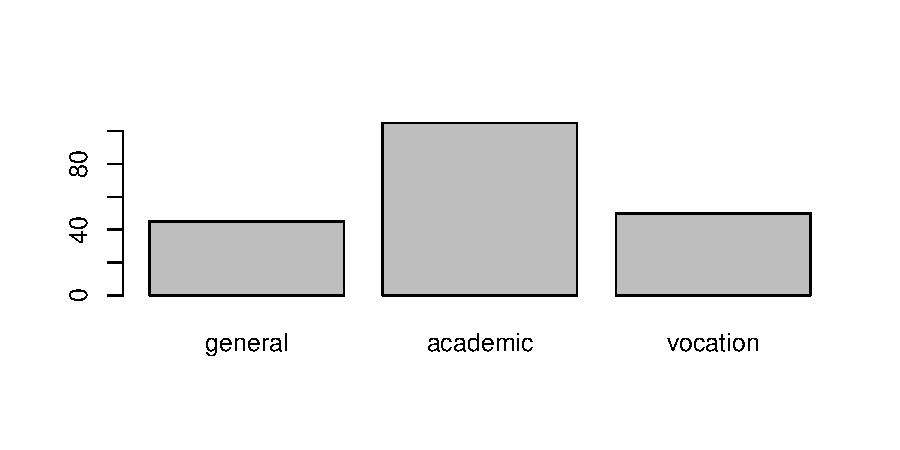
\includegraphics[width=\maxwidth]{figure/hist-1} 

}



\end{knitrout}

Expliquemos un poco de qu\'e se tratan estos programas que se dan en Estados Unidos:

\begin{enumerate}
	\item ``{\bf general}'': programas universitarios que conducen hacia la primera mitad de una licenciatura (tipo bachillerato).
	\item ``{\bf academic}'': programas universitarios que conducen hacia el final una licenciatura (como tu programa, o el que estudi\'e yo en pregrado).
	\item ``{\bf vocational}'': programas t\'ecnicos. 
\end{enumerate}


El paquete de \texttt{R} que usaremos se llama \texttt{nnet}---\'este especifica que la variable dependiente debe ser \texttt{factor}. Adem\'as, debemos escoger la categor\'ia de referencia:

\begin{knitrout}
\definecolor{shadecolor}{rgb}{0.969, 0.969, 0.969}\color{fgcolor}\begin{kframe}
\begin{alltt}
\hlkwd{is}\hlstd{(dat}\hlopt{$}\hlstd{prog)[}\hlnum{1}\hlstd{]} \hlcom{# ok, es factor}
\end{alltt}
\begin{verbatim}
## [1] "factor"
\end{verbatim}
\begin{alltt}
\hlstd{dat}\hlopt{$}\hlstd{prog2} \hlkwb{<-} \hlkwd{relevel}\hlstd{(dat}\hlopt{$}\hlstd{prog,} \hlkwc{ref} \hlstd{=} \hlstr{"academic"}\hlstd{)} \hlcom{# ref cat}
\end{alltt}
\end{kframe}
\end{knitrout}


Ahora estimemos el modelo,

\begin{knitrout}
\definecolor{shadecolor}{rgb}{0.969, 0.969, 0.969}\color{fgcolor}\begin{kframe}
\begin{alltt}
\hlkwd{p_load}\hlstd{(nnet)}
\hlstd{modelo} \hlkwb{<-} \hlkwd{multinom}\hlstd{(prog2} \hlopt{~} \hlstd{ses} \hlopt{+} \hlstd{write,} \hlkwc{data} \hlstd{= dat)}
\end{alltt}
\begin{verbatim}
## # weights:  15 (8 variable)
## initial  value 219.722458 
## iter  10 value 179.982880
## final  value 179.981726 
## converged
\end{verbatim}
\end{kframe}
\end{knitrout}

Hagamos una tabla.

\begin{kframe}
\begin{alltt}
\hlkwd{p_load}\hlstd{(texreg)}
\hlkwd{texreg}\hlstd{(modelo)} \hlcom{# usa "screenreg" no "texreg".}
\end{alltt}
\end{kframe}
\begin{table}
\begin{center}
\begin{tabular}{l c}
\hline
 & Model 1 \\
\hline
general: (Intercept)  & $2.85^{*}$    \\
                      & $(1.17)$      \\
general: sesmiddle    & $-0.53$       \\
                      & $(0.44)$      \\
general: seshigh      & $-1.16^{*}$   \\
                      & $(0.51)$      \\
general: write        & $-0.06^{**}$  \\
                      & $(0.02)$      \\
vocation: (Intercept) & $5.22^{***}$  \\
                      & $(1.16)$      \\
vocation: sesmiddle   & $0.29$        \\
                      & $(0.48)$      \\
vocation: seshigh     & $-0.98$       \\
                      & $(0.60)$      \\
vocation: write       & $-0.11^{***}$ \\
                      & $(0.02)$      \\
\hline
AIC                   & $375.96$      \\
BIC                   & $402.35$      \\
Log Likelihood        & $-179.98$     \\
Deviance              & $359.96$      \\
Num. obs.             & $200$         \\
K                     & $3$           \\
\hline
\multicolumn{2}{l}{\scriptsize{$^{***}p<0.001$; $^{**}p<0.01$; $^{*}p<0.05$}}
\end{tabular}
\caption{Statistical models}
\label{table:coefficients}
\end{center}
\end{table}


Lo que acabamos de estimar tiene un correlato en la parte te\'orica que acabamos de discutir en \autoref{fruta}.


\begin{equation}
\begin{split}
ln[\frac{\text{Pr}(\text{program: general})}{Pr(\text{program: academic})}]  = \beta_{10} + \beta{11}(\text{ses}=\text{middle}) + \beta_{12}(\text{ses}=\text{high}) + \beta_{13}\text{(write)}\\
ln[\frac{\text{Pr}(\text{program: vocation})}{Pr(\text{program: academic})}] = \beta_{20} + \beta{22}(\text{ses}=\text{middle}) + \beta_{22}(\text{ses}=\text{high}) + \beta_{23}\text{(write)}
\end{split}
\end{equation}

O lo que en n\'umeros es (tomando los resultados de la tabla),

\begin{equation}\label{inter}
\begin{split}
ln[\frac{\text{Pr}(\text{program: general})}{Pr(\text{program: academic})}]  = 2.85 -0.53(\text{ses}=\text{middle})  -1.16(\text{ses}=\text{high}) -0.06\text{(write)}\\
ln[\frac{\text{Pr}(\text{program: vocation})}{Pr(\text{program: academic})}] = 5.22 + 0.29(\text{ses}=\text{middle}) -0.98(\text{ses}=\text{high}) -0.11\text{(write)}
\end{split}
\end{equation}


 



\section{Interpretaci\'on} 

Ahora interpretaremos el modelo. Tomando la \autoref{inter}, se interpreta como siempre. Por ejemplo, el $\beta_{13}$ significa, cuando \texttt{write} sube una unidad, los {\bf log-odds} de estar en un programa \texttt{general} {\bf versus} un programa \texttt{academic} decrecen -0.06. Otro ejemplo es el $\beta_{11}$: cuando subo en una unidad \texttt{ses} (es decir de \texttt{low} a \texttt{middle}), los {\bf log-odds} de estar en un programa \texttt{general} {\bf versus} un programa \texttt{academic} decrecen -0.53.

Este modelo es bastante complejo. No solo en su parametrizaci\'on (\autoref{pmf.mlogit}), sino que tambi\'en en su interpretaci\'on (\autoref{inter}). Es por esto que nos saltaremos los \emph{odds rations} y los cambios marginales. Todos ellos est\'an en escala de log-ods, dificultando aun m\'as la interpretaci\'on substantiva de la tabla de regresi\'on. Es por esto que saltaremos directo a las \emph{predicted probabilities}. La ventaja es que podremos calcular todas las probabilidades, \emph{incluso de la categor\'ia base}. 

\begin{kframe}
\begin{alltt}
\hlkwd{p_load}\hlstd{(effects)}
\hlkwd{plot}\hlstd{(}\hlkwd{effect}\hlstd{(}\hlstr{"ses"}\hlstd{, modelo))}
\end{alltt}
\end{kframe}

{\centering 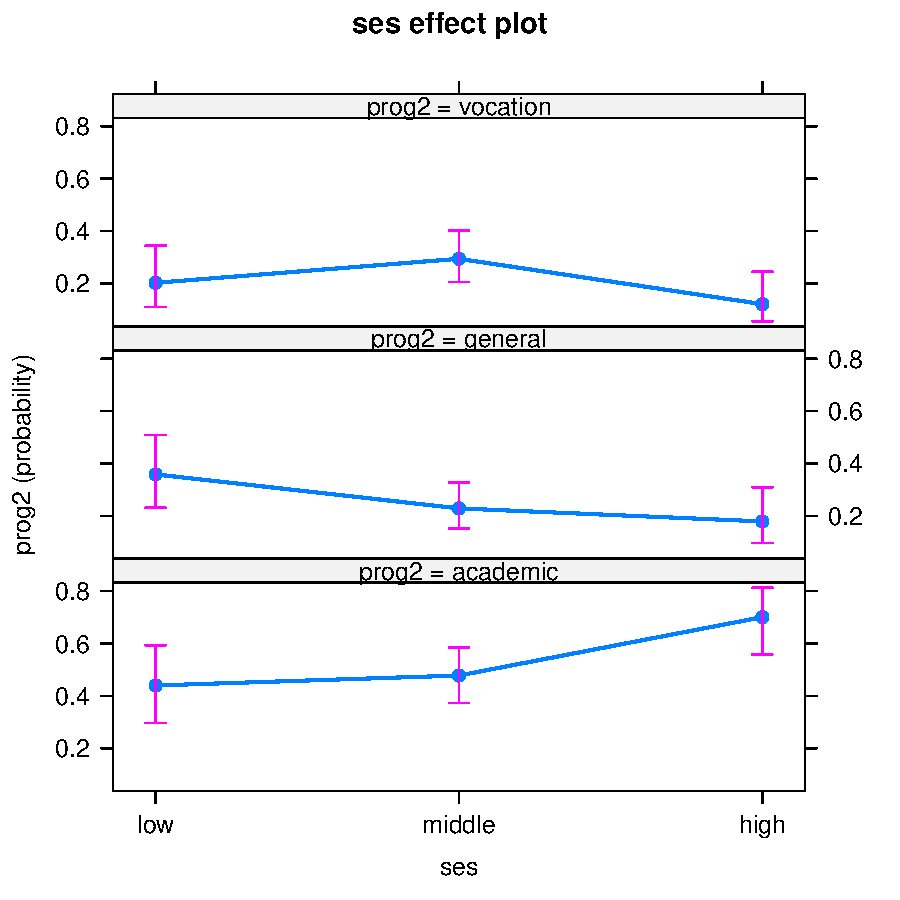
\includegraphics[width=\maxwidth]{figure/pp-1} 

}


\begin{kframe}\begin{alltt}
\hlkwd{plot}\hlstd{(}\hlkwd{effect}\hlstd{(}\hlstr{"write"}\hlstd{, modelo))}
\end{alltt}
\end{kframe}

{\centering 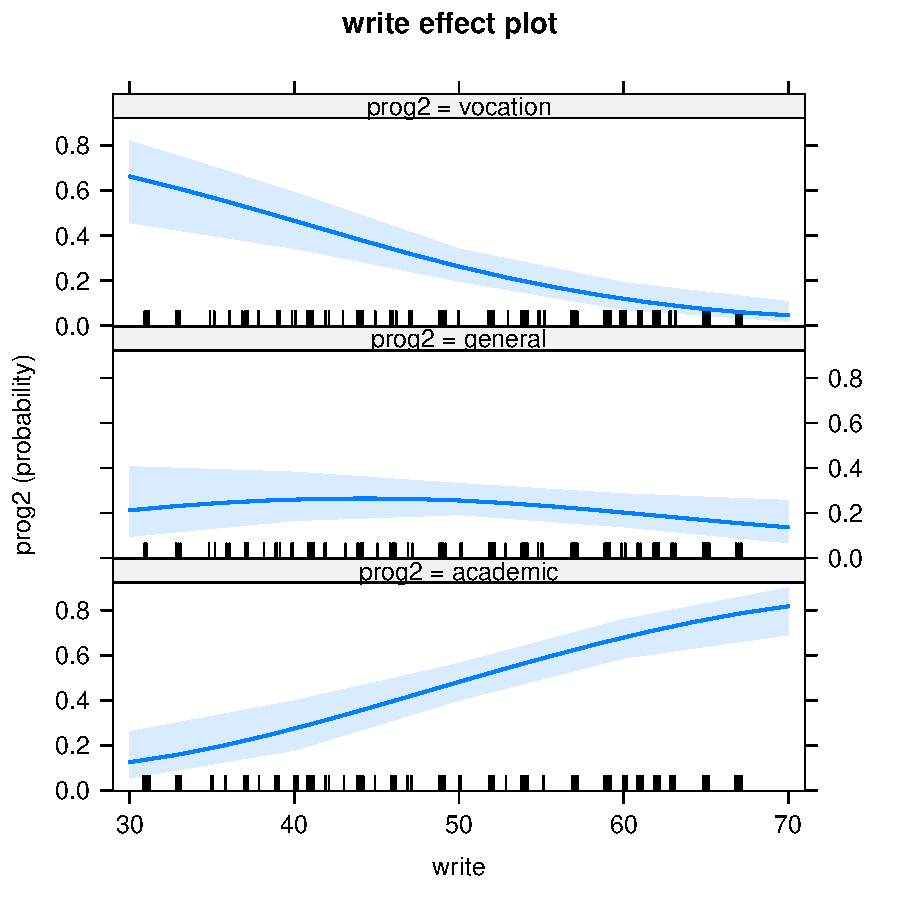
\includegraphics[width=\maxwidth]{figure/pp-2} 

}




Algunos ejemplos de interpretaci\'on:

\begin{enumerate}
	\item Estudiantes con \emph{background} socio-econ\'omico (\texttt{ses}) {\bf alto} tienden a preferir programas \texttt{academic}.
	\item Estudiantes con \emph{background} socio-econ\'omico (\texttt{ses}) {\bf bajo} tienden a preferir programas \texttt{general}.
	\item Estudiantes que logran puntajes {\bf altos} en la prueba de escritura (\texttt{write}) tienden a preferir programas \texttt{academic}.
	\item Estudiantes que logran puntajes {\bf bajos} en la prueba de escritura (\texttt{write}) tienden a preferir programas \texttt{vocation}.
\end{enumerate}


\paragraph{IIA} Veamos si el supuesto IIA se cumple.





\begin{knitrout}
\definecolor{shadecolor}{rgb}{0.969, 0.969, 0.969}\color{fgcolor}\begin{kframe}
\begin{alltt}
\hlstd{knitr}\hlopt{::}\hlkwd{purl}\hlstd{(}\hlstr{'Multinomial.Rnw'}\hlstd{)}
\end{alltt}


{\ttfamily\noindent\bfseries\color{errorcolor}{\#\# Error in parse\_block(g[-1], g[1], params.src, markdown\_mode): Duplicate chunk label 'setup', which has been used for the chunk:\\\#\# if (!require("{}pacman"{})) install.packages("{}pacman"{}); library(pacman)\\\#\# p\_load(knitr)\\\#\# set.seed(2020)\\\#\# options(scipen=9999999)}}\begin{alltt}
\hlkwd{Stangle}\hlstd{(}\hlstr{'Multinomial.Rnw'}\hlstd{)}
\end{alltt}
\begin{verbatim}
## Writing to file Multinomial.R
\end{verbatim}


{\ttfamily\noindent\bfseries\color{errorcolor}{\#\# Error in match.arg(options\$results, c("{}verbatim"{}, "{}tex"{}, "{}hide"{})): 'arg' should be one of "{}verbatim"{}, "{}tex"{}, "{}hide"{}}}\end{kframe}
\end{knitrout}


%\newpage
%\paragraph{}
%\paragraph{}
%\pagenumbering{Roman}
%\setcounter{page}{1}
%\printbibliography



\end{document}
